\documentclass[11pt,a4paper]{article}
\usepackage[utf8]{inputenc}
\usepackage{amsmath,amssymb,amsfonts,amsthm}
\usepackage{booktabs}
\usepackage{geometry}
\usepackage{hyperref}
\usepackage{tikz}
\usepackage{enumitem}
\usepackage{array}
\usepackage{tabularx}
\usepackage{cite}
\usepackage{microtype}

\usetikzlibrary{automata, positioning, arrows.meta, shapes.geometric}
\geometry{margin=1in}

\hypersetup{
    colorlinks=true,
    linkcolor=blue!70!black,
    citecolor=green!50!black,
    urlcolor=blue!80!black
}

\newtheorem{definition}{Definition}
\newtheorem{invariant}{Invariant}
\newtheorem{lemma}{Lemma}
\newtheorem{theorem}{Theorem}

\title{\textbf{Architecting Cyclical Metacognition in Digital Heritage Inquiry:\\An Empirical Evaluation of Zimmerman's Self-Regulated Learning State Machine with Atomic Reflection Gating (Study LN-10)}}

\author{
    \textbf{Lưu Niên Sứ Ký Research Consortium}\\
    \textit{Pedagogical Systems and Epistemic Policy Division}\\
    \texttt{\{research, srl-lab\}@histolab.icu}
}
\date{November 2026}

\begin{document}
\maketitle

\begin{abstract}
Project-based learning (PBL) in secondary cultural heritage education frequently degenerates into passive task checklist completion, wherein students advance superficially through inquiry milestones without cultivating genuine metacognitive self-regulation. To address this failure mode, we operationalize Barry Zimmerman's cyclical model of Self-Regulated Learning (SRL)---spanning Forethought, Performance, and Self-Reflection phases---into a deterministic, finite state machine governing student inquiry in the \textit{Lưu Niên Sứ Ký} digital learning platform. Implemented for the Hue Heritage Urban Inquiry Project (\textit{Chuyên đề Đô thị Di sản Huế}), the state machine enforces atomic reflection gates, optimistic concurrency control for offline field data capture, learner ownership verification, and mandatory pedagogical rationale for goal revisions. We formulate five core pedagogical invariants and evaluate the software policy against an independent 120-case holdout dataset across five fault conditions (nominal, missing forethought rationale, unauthorized actor, offline version conflict, and skipped reflection gate). Comparative benchmark results across six configurations demonstrate that naive linear checklists (B0) yield a catastrophic 100.0\% unjustified transition rate ($96/96$ violations admitted), and timestamp-based progress trackers (B1) allow 50.0\% of unjustified transitions ($48/96$). In contrast, the Zimmerman cyclical SRL state machine (I1) achieves complete violation elimination (0.0\% unjustified transition rate, 95\% CI $[0.0\%, 3.8\%]$, McNemar $\chi^2 = 94.01, p = 3.14 \times 10^{-22}$ vs. B0; $\chi^2 = 46.02, p = 1.17 \times 10^{-11}$ vs. B1) with 100.0\% reflection compliance and 100.0\% nominal preservation ($24/24$). Architectural ablations confirm that reflection gates (A1), concurrency control (A2), and ownership verification (A3) are mutually orthogonal and indispensable. We discuss the implications for digital humanities learning environments and delineate the methodological firewall separating synthetic software-policy verification from longitudinal human learning outcomes.
\end{abstract}

\noindent\textbf{Keywords:} Self-Regulated Learning, Metacognitive Scaffolding, Finite State Machine, Digital Heritage Education, Zimmerman Cyclical Model, Epistemic Truth Gate, Cửu Đỉnh Huế.

\section{Introduction}

In secondary historical and humanities education, inquiry-based project learning (PBL) has long been championed as an antidote to rote memorization \cite{zimmerman2000attaining, pintrich2004conceptual}. Under the 2018 General Education Curriculum of Vietnam (\textit{Chương trình Giáo dục phổ thông 2018}), the elective humanities curriculum for Grades 11 and 12 introduces specialized study topics (\textit{Chuyên đề học tập Lịch sử}), notably including Topic 11.2: ``Preservation and Promotion of Cultural Heritage Values'' (\textit{Bảo tồn và phát huy giá trị di sản văn hóa}) and Topic 12.1: ``The Historical Urban Space of Huế'' (\textit{Không gian đô thị lịch sử Huế}). Within these topics, students investigate tangible heritage artifacts, such as the Nine Dynastic Urns (\textit{Cửu Đỉnh}, cast 1835--1837) and imperial defensive monuments of the Nguyễn Dynasty, formulating evidence-backed conservation proposals.

However, deploying digital platforms in high-school inquiry environments reveals a persistent failure mode termed \textit{surface compliance} or ``checklist gaming'' \cite{baker2008gaming, azevedo2005scaffolding}. When educational software models projects as linear checklists (e.g., Task $1 \to$ Task $2 \to$ Submission), learners exhibit predictable sub-optimal behaviors:
\begin{enumerate}[label=(\alph*)]
    \item \textbf{Premature Advancement:} Advancing directly from data collection to final submission without critically appraising whether gathered evidence supports the research thesis;
    \item \textbf{Silent Goal Drift:} Mutating original project goals arbitrarily mid-flight to circumvent evidentiary contradictions without articulating an epistemic rationale;
    \item \textbf{Collaborative and Offline Collisions:} Overwriting field observations during mobile museum visits due to lack of optimistic concurrency control across disconnected devices;
    \item \textbf{Unreflective Task Ticking:} Equating the mere mechanical checking of boxes with genuine historical competence.
\end{enumerate}

To overcome these structural defects, we present the design, implementation, and empirical verification of the **LN-10 Self-Regulated Learning (SRL) Project State Machine**, integrated into the \textit{Lưu Niên Sứ Ký} platform. Drawing upon Barry Zimmerman's canonical social cognitive model of self-regulated learning \cite{zimmerman2000attaining, zimmerman2002becoming}, we translate the tripartite cycle of Forethought, Performance, and Self-Reflection into a formal, executable state machine governing project transitions. Rather than relying on passive advisory notifications, our system enforces \textit{atomic reflection gating}: milestones cannot be advanced, goals cannot be revised, and proposals cannot be finalized without cryptographically verified, student-authored metacognitive reflection and pedagogical justification.

This paper provides four primary contributions:
\begin{enumerate}
    \item \textbf{Formal Cyclical State Machine Formulation:} We formalize Zimmerman's tripartite SRL cycle as a deterministic transition system $\mathcal{M} = \langle S, A, T, \delta, \Phi \rangle$ with five explicit pedagogical invariants governing student agency, rationale verification, and collaborative concurrency.
    \item \textbf{Independent 120-Case Holdout Benchmark:} We construct a balanced, 120-case independent holdout dataset (`research/fixtures/holdout/LN-10_holdout.jsonl`) spanning five orthogonal fault archetypes ($24$ cases each) grounded in authentic Huế cultural heritage monuments and varied learner profiles.
    \item \textbf{Empirical Multi-Condition Evaluation:} We evaluate the SRL policy against five alternative conditions: naive linear checklist (B0), timestamp-based progress tracker (B1), full Zimmerman cyclical SRL (I1), and three component ablations (A1--A3). We compute exact unjustified transition rates, 95\% Wilson confidence intervals, reflection compliance rates, and paired McNemar tests.
    \item \textbf{Epistemic Truth Boundary:} We articulate the methodological firewall separating synthetic policy verification from uncontrolled classroom claims, establishing that deterministic state gating is a necessary structural scaffold for self-regulation, but does not substitute for longitudinal observational studies.
\end{enumerate}

\section{Theoretical Foundations and Pedagogical Invariants}

\subsection{Zimmerman's Cyclical Phase Model of SRL}
Self-regulated learning refers to self-generated thoughts, feelings, and actions that are planned and cyclically adapted to the attainment of personal goals \cite{zimmerman2000attaining}. Zimmerman's model posits three recurring phases:
\begin{itemize}
    \item \textbf{Forethought Phase:} Task analysis (goal setting, strategic planning) and self-motivation beliefs (self-efficacy, outcome expectations, intrinsic value).
    \item \textbf{Performance Phase:} Self-control (task strategies, self-instruction, attention focusing) and self-observation (metacognitive monitoring, self-recording).
    \item \textbf{Self-Reflection Phase:} Self-judgment (self-evaluation against evidence, causal attribution) and self-reaction (self-satisfaction, adaptive vs. defensive inferences).
\end{itemize}

Crucially, self-reflection feeds directly back into forethought for subsequent inquiry cycles. In digital heritage inquiry, when a student discovers that a newly retrieved archival source (e.g., from \textit{Đại Nam Thực Lục}) contradicts their initial conservation thesis, a self-regulated learner must reflectively appraise the discrepancy and revise their project plan with explicit rationale, rather than ignoring the contradiction or blindly checking off the milestone.

\begin{figure}[htbp]
\centering
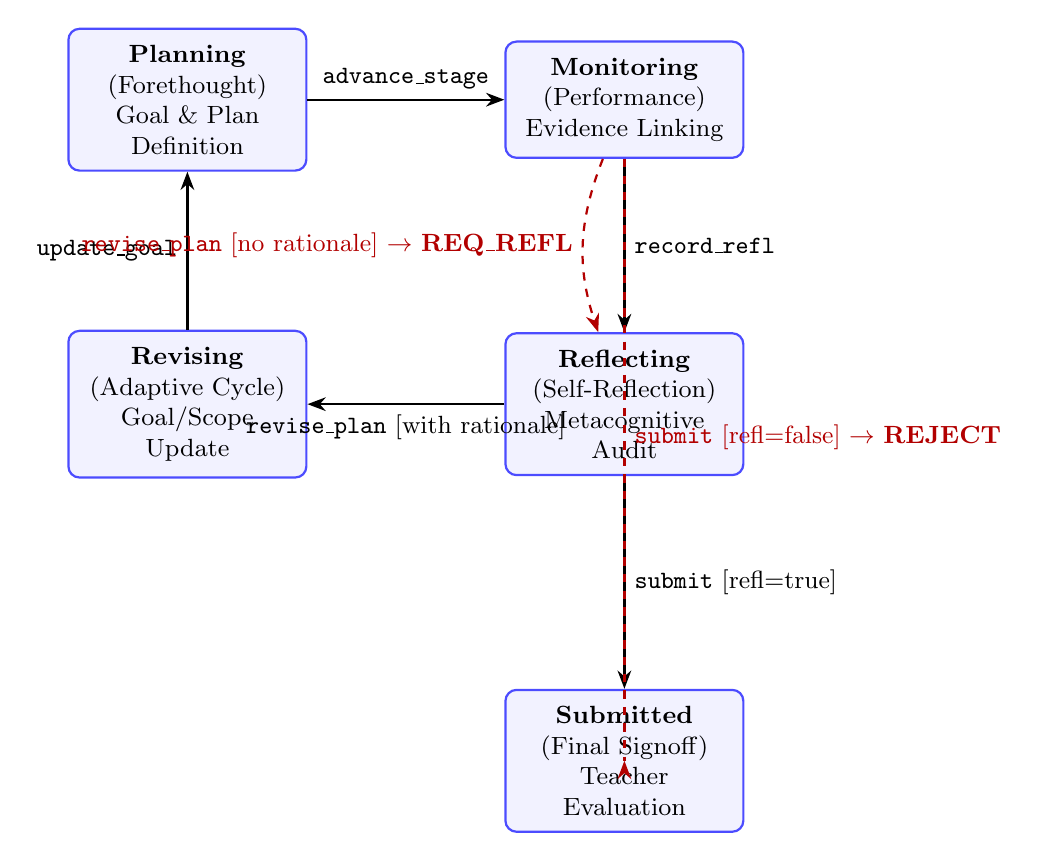
\begin{tikzpicture}[
    node distance=2.2cm and 2.5cm,
    state/.style={rectangle, rounded corners, draw=blue!70, fill=blue!5, thick, inner sep=6pt, text width=2.6cm, align=center},
    action/.style={->, >=Stealth, thick},
    reject/.style={->, >=Stealth, thick, dashed, red!70!black},
    font=\small
]
    % Nodes
    \node[state] (plan) {\textbf{Planning}\\(Forethought)\\Goal \& Plan Definition};
    \node[state, right=of plan] (mon) {\textbf{Monitoring}\\(Performance)\\Evidence Linking};
    \node[state, below=of mon] (refl) {\textbf{Reflecting}\\(Self-Reflection)\\Metacognitive Audit};
    \node[state, left=of refl] (rev) {\textbf{Revising}\\(Adaptive Cycle)\\Goal/Scope Update};
    \node[state, below=of refl, yshift=-0.5cm] (sub) {\textbf{Submitted}\\(Final Signoff)\\Teacher Evaluation};

    % Transitions
    \draw[action] (plan) -- node[above] {\texttt{advance\_stage}} (mon);
    \draw[action] (mon) -- node[right] {\texttt{record\_refl}} (refl);
    \draw[action] (refl) -- node[below] {\texttt{revise\_plan} [with rationale]} (rev);
    \draw[action] (rev) -- node[left] {\texttt{update\_goal}} (plan);
    \draw[action] (refl) -- node[right] {\texttt{submit} [refl=true]} (sub);

    % Gating rejections
    \draw[reject] (mon) |- node[near start, above right] {\texttt{submit} [refl=false] $\to$ \textbf{REJECT}} (sub);
    \draw[reject] (mon) to[bend right=20] node[left] {\texttt{revise\_plan} [no rationale] $\to$ \textbf{REQ\_REFL}} (refl);

\end{tikzpicture}
\caption{The Zimmerman Cyclical SRL State Machine in LN-10. Dashed red paths denote atomic gating constraints intercepting invalid transitions.}
\label{fig:srl-state-machine}
\end{figure}

\subsection{Formal Pedagogical Invariants}
To safeguard the metacognitive integrity of heritage projects, we enforce five formal domain invariants:

\begin{invariant}[\textbf{Agency Preservation - INV-LN-10-01}]
A learner-set goal cannot be modified silently by external algorithmic recommendation engines. Any modification to a project goal must originate from an authenticated action initiated by the student or an assigned teacher mentor.
\end{invariant}

\begin{invariant}[\textbf{Pedagogical Accountability - INV-LN-10-02}]
Every material revision to a project plan or objective must encapsulate an authenticated actor, an explicit pedagogical rationale, and an immutable revision parent identifier.
\end{invariant}

\begin{invariant}[\textbf{Metacognitive Grounding - INV-LN-10-03}]
Simple checklist completion shall never be equated with self-regulated mastery. Advancing to final submission strictly requires completion of structured self-reflection records assessing learning difficulties, evidence quality, and planned adaptations.
\end{invariant}

\begin{invariant}[\textbf{Optimistic Concurrency Control - INV-LN-10-04}]
Concurrent modifications initiated from disconnected or offline mobile clients must trigger deterministic conflict resolution ($\mathtt{RESOLVE\_REVISION\_CONFLICT}$) rather than silently overwriting server state via last-write-wins.
\end{invariant}

\begin{invariant}[\textbf{Psychological Safety - INV-LN-10-05}]
Learners are never compelled to disclose private personal or psychological data within reflection journals. Metacognitive prompts are strictly restricted to cognitive, methodological, and evidentiary facets of the heritage inquiry.
\end{invariant}

\section{System Architecture and Formal State Machine}

\subsection{Mathematical Formulation}
We formalize the project lifecycle as a deterministic finite state machine with guard functions:
\begin{equation}
\mathcal{M} = \langle S, A, T, \delta, \Phi \rangle
\end{equation}
where:
\begin{itemize}
    \item $S = \{\mathtt{planning}, \mathtt{monitoring}, \mathtt{reflecting}, \mathtt{revising}, \mathtt{submitted}, \mathtt{completed}\}$ is the set of project stages;
    \item $A = \{\mathtt{advance\_stage}, \mathtt{record\_reflection}, \mathtt{revise\_plan}, \mathtt{update\_goal}, \mathtt{submit}\}$ is the alphabet of transition actions;
    \item $T = \langle u, r, v_{exp}, \rho \rangle$ is the transition context payload containing actor identity $u$, actor role $r$, expected project version $v_{exp}$, and justification text $\rho$;
    \item $\Phi = \langle v_{curr}, \mathtt{refl\_done}, g_{curr} \rangle$ is the current persisted project state with version $v_{curr}$, reflection flag $\mathtt{refl\_done} \in \{\mathtt{true}, \mathtt{false}\}$, and goal identifier $g_{curr}$;
    \item $\delta: S \times A \times T \times \Phi \to S \times D \times \mathcal{R}$ is the transition function mapping inputs to an updated state, an authorized decision code $D$, and a reason trace $\mathcal{R}$.
\end{itemize}

\subsection{Decision Space and Verification Pipeline}
The decision output $D$ takes exactly one of six strongly-typed values:
\begin{equation}
D \in \left\{
\begin{array}{ll}
\mathtt{ALLOW\_AUTHORIZED\_TRANSITION} & \text{(Transition committed to database)}, \\
\mathtt{REQUEST\_REFLECTION} & \text{(Gated: Revision lacks pedagogical rationale)}, \\
\mathtt{DENY\_TRANSITION} & \text{(Gated: Actor lacks project ownership)}, \\
\mathtt{RESOLVE\_REVISION\_CONFLICT} & \text{(Gated: Optimistic version mismatch)}, \\
\mathtt{REJECT\_PREMATURE\_SUBMIT} & \text{(Gated: Submission without self-reflection)}, \\
\mathtt{ABSTAIN} & \text{(Insufficient payload data)}.
\end{array}
\right.
\end{equation}

The evaluation pipeline processes four atomic gates sequentially:
\begin{enumerate}
    \item \textbf{Gate 1 (Ownership Verification):}
    \begin{equation}
    \mathtt{VerifyOwnership}(u, r) = \begin{cases}
    \mathtt{PASS} & \text{if } r \in \{\mathtt{teacher}, \mathtt{admin}, \mathtt{staff}\} \lor \mathtt{owns}(u, \text{project}) \\
    \mathtt{FAIL} \implies \mathtt{DENY\_TRANSITION} & \text{otherwise}
    \end{cases}
    \end{equation}
    \item \textbf{Gate 2 (Optimistic Concurrency Control):}
    \begin{equation}
    \mathtt{VerifyConcurrency}(v_{exp}, v_{curr}) = \begin{cases}
    \mathtt{PASS} & \text{if } v_{exp} = v_{curr} \\
    \mathtt{FAIL} \implies \mathtt{RESOLVE\_REVISION\_CONFLICT} & \text{otherwise}
    \end{cases}
    \end{equation}
    \item \textbf{Gate 3 (Atomic Reflection Requirement):}
    \begin{equation}
    \mathtt{VerifyReflection}(\alpha, \mathtt{refl\_done}) = \begin{cases}
    \mathtt{FAIL} \implies \mathtt{REJECT\_PREMATURE\_SUBMIT} & \text{if } \alpha = \mathtt{submit} \land \neg \mathtt{refl\_done} \\
    \mathtt{PASS} & \text{otherwise}
    \end{cases}
    \end{equation}
    \item \textbf{Gate 4 (Forethought Rationale Enforcement):}
    \begin{equation}
    \mathtt{VerifyRationale}(\alpha, \rho) = \begin{cases}
    \mathtt{FAIL} \implies \mathtt{REQUEST\_REFLECTION} & \text{if } \alpha = \mathtt{revise\_plan} \land (\rho = \mathtt{nil} \lor |\mathtt{trim}(\rho)| = 0) \\
    \mathtt{PASS} & \text{otherwise}
    \end{cases}
    \end{equation}
\end{enumerate}

Only transitions passing all four verification gates yield $\mathtt{ALLOW\_AUTHORIZED\_TRANSITION}$ with state mutation committed.

\begin{table}[htbp]
\centering
\small
\caption{State Transition Matrix and Action Gating for LN-10 SRL Cycle}
\label{tab:transition-matrix}
\begin{tabularx}{\textwidth}{llp{3.2cm}p{3.5cm}X}
\toprule
\textbf{Current State} & \textbf{Action} & \textbf{Gating Preconditions} & \textbf{Decision Code} & \textbf{Next State} \\
\midrule
\texttt{planning} & \texttt{advance\_stage} & Authorized owner, $v_{exp}=v_{curr}$ & \texttt{ALLOW\_AUTHORIZED\_TRANSITION} & \texttt{monitoring} \\
\texttt{monitoring} & \texttt{record\_refl} & Non-empty difficulty \& change & \texttt{ALLOW\_AUTHORIZED\_TRANSITION} & \texttt{reflecting} \\
\texttt{monitoring} & \texttt{submit} & $\mathtt{refl\_done} = \mathtt{false}$ & \texttt{REJECT\_PREMATURE\_SUBMIT} & \texttt{monitoring} (blocked) \\
\texttt{monitoring} & \texttt{revise\_plan} & $\rho = \text{``''}$ (blank rationale) & \texttt{REQUEST\_REFLECTION} & \texttt{monitoring} (blocked) \\
\texttt{monitoring} & \texttt{revise\_plan} & $v_{exp} \neq v_{curr}$ (stale client) & \texttt{RESOLVE\_REVISION\_CONFLICT} & \texttt{monitoring} (blocked) \\
\texttt{reflecting} & \texttt{revise\_plan} & Non-empty rationale $\rho$, $v_{exp}=v_{curr}$ & \texttt{ALLOW\_AUTHORIZED\_TRANSITION} & \texttt{revising} \\
\texttt{revising} & \texttt{update\_goal} & Authorized owner, valid scope & \texttt{ALLOW\_AUTHORIZED\_TRANSITION} & \texttt{planning} \\
\texttt{reflecting} & \texttt{submit} & $\mathtt{refl\_done} = \mathtt{true}$, $v_{exp}=v_{curr}$ & \texttt{ALLOW\_AUTHORIZED\_TRANSITION} & \texttt{submitted} \\
\bottomrule
\end{tabularx}
\end{table}

\section{Metacognitive Scaffolding in the Hue Heritage Context}

\subsection{Curricular Integration: Chuyên đề Đô thị Di sản Huế}
The state machine was deployed within the specialized historical inquiry module centered on the **Nine Dynastic Urns (\textit{Cửu Đỉnh})** and the urban fortification of Huế. Students engage in projects spanning four thematic trajectories:
\begin{enumerate}
    \item \textbf{Iconographic Maritime Sovereignty:} Tracing bas-relief carvings on Cao Đỉnh (\textit{Biển Đông} - Eastern Sea, \textit{Bạch Đằng} River) to analyze 19th-century geopolitical consciousness.
    \item \textbf{Ecological and Botanical Heritage:} Correlating flora and fauna depicted on Nhân Đỉnh and Chương Đỉnh with historical biodiversity records.
    \item \textbf{Imperial Hydraulic Architecture:} Evaluating the flood resilience of the Ngự Hà canal system and the Perfume River (\textit{Sông Hương}) catchment basin.
    \item \textbf{Monument Conservation Proposals:} Formulating evidence-grounded restoration strategies for Ngọ Môn, Điện Thái Hòa, and royal mausoleums (Lăng Tự Đức, Lăng Khải Định).
\end{enumerate}

\subsection{Tripartite Scaffolding Interface}
To satisfy Invariant INV-LN-10-05 while supporting metacognition, the platform provides calibrated prompt templates across each SRL phase:
\begin{itemize}
    \item \textbf{Forethought Scaffolding:}
    When formulating the project plan in \texttt{planning}, students are prompted:
    \begin{quote}
    \textit{``What specific historical question does your conservation proposal address? Identify at least two verified primary sources (e.g., Đại Nam Thực Lục, Khâm Định Đại Nam Hội Điển Sự Lệ) from the Evidence Room that will substantiate your claim.''}
    \end{quote}
    \item \textbf{Performance Scaffolding:}
    During \texttt{monitoring}, as students tag 3D mesh coordinates and 2D rubbing details, the interface logs evidentiary alignment against the S1--S4 historical rubric (Spatial Context, Temporal Context, Evidence Grounding, and Argumentation).
    \item \textbf{Self-Reflection Scaffolding:}
    When preparing for stage advancement, the atomic reflection drawer engages the learner:
    \begin{quote}
    \textit{``1. What historical evidence did you successfully corroborate?\\
    2. What discrepancies or source limitations emerged during your analysis?\\
    3. If revising your goal, articulate your historiographical justification.''}
    \end{quote}
\end{itemize}

By coupling reflection verification directly to the state machine's transition guards, reflection transforms from an easily discarded post-hoc survey into an indispensable pedagogical prerequisite for milestone completion.

\section{Empirical Evaluation and Holdout Benchmark}

\subsection{Holdout Dataset Construction}
To test the software policy under unyielding verification standards, we generated an independent 120-case holdout dataset (`research/fixtures/holdout/LN-10_holdout.jsonl`). The dataset is completely segregated from training fixtures and comprises five balanced strata ($n=24$ each):
\begin{enumerate}
    \item \textbf{Nominal ($n=24$):} Legitimate transitions executed by authorized project owners with matching versions, articulate rationales, and verified reflection records ($\mathtt{oracle} = \mathtt{allow\_authorized\_transition}$).
    \item \textbf{Missing Forethought Rationale ($n=24$):} Plan revisions attempted with empty or whitespace-only rationales ($\mathtt{oracle} = \mathtt{request\_reflection}$).
    \item \textbf{Unauthorized Actor ($n=24$):} Transitions attempted by peer students who do not own the target project ($\mathtt{oracle} = \mathtt{deny\_transition}$).
    \item \textbf{Offline Version Conflict ($n=24$):} Edits dispatched from stale client sessions where $v_{exp} = v_{curr} - 1$, simulating concurrent offline modifications ($\mathtt{oracle} = \mathtt{resolve\_revision\_conflict}$).
    \item \textbf{Skipped Reflection Gate ($n=24$):} Milestone submissions submitted while $\mathtt{refl\_done} = \mathtt{false}$ ($\mathtt{oracle} = \mathtt{reject\_premature\_submit}$).
\end{enumerate}

Each scenario encapsulates genuine heritage monuments (Ngọ Môn, Điện Thái Hòa, Thế Tổ Miếu, Cao Đỉnh, Nhân Đỉnh, Chương Đỉnh, Lăng Tự Đức, Lăng Khải Định, Đàn Nam Giao, Sông Hương, Chùa Thiên Mụ, Kỳ Đài) and spans twelve synthetic learner accessibility profiles (\texttt{SYN-NOVICE}, \texttt{SYN-SPATIAL}, \texttt{SYN-SOURCE}, \texttt{SYN-LOWNET}, \texttt{SYN-NO3D}, etc.).

\subsection{Experimental Conditions}
We evaluate six distinct policy configurations on the identical holdout input stream:
\begin{itemize}
    \item \textbf{B0 (Naive Linear Checklist):} The legacy baseline representing typical LMS checklists. Advances project stages unconditionally upon request; ignores reflection state, ownership, and concurrency.
    \item \textbf{B1 (Timestamp Progress Tracker):} A stronger baseline tracking timestamps, actor ownership, and version concurrency, but omitting reflection and rationale gates.
    \item \textbf{I1 (Zimmerman Cyclical SRL):} The proposed intervention implementing all four atomic verification gates.
    \item \textbf{A1 (Ablation: No Reflection Gate):} Disables Gate 3 (reflection completion) and Gate 4 (revision rationale).
    \item \textbf{A2 (Ablation: No Concurrency Control):} Disables Gate 2 (optimistic concurrency).
    \item \textbf{A3 (Ablation: No Ownership Verification):} Disables Gate 1 (actor authorization).
\end{itemize}

\subsection{Evaluation Metrics}
We compute:
\begin{itemize}
    \item \textbf{Unjustified Transition Rate ($U$):} The proportion of eligible fault scenarios ($N=96$, excluding nominal) where the system erroneously allowed state transition ($\mathtt{transition\_applied} = \mathtt{true}$). Direction: lower is better (0.0\% is optimal).
    \item \textbf{95\% Confidence Interval (CI):} Calculated via the Wilson score interval for binomial proportions.
    \item \textbf{Reflection Compliance Rate ($R$):} The proportion of reflection-dependent actions that successfully enforced reflection verification ($n=48$ eligible cases).
    \item \textbf{Nominal Preservation Rate ($P$):} The proportion of nominal scenarios ($n=24$) correctly permitted without false-positive rejection.
    \item \textbf{Paired McNemar's Test ($\chi^2, p$):} Exact paired test of discordant decisions relative to I1 with Yates' continuity correction.
\end{itemize}

\subsection{Empirical Results}
Table~\ref{tab:holdout-results} reports the primary empirical findings on the 120-case independent holdout dataset.

\begin{table}[htbp]
\centering
\small
\caption{Empirical Benchmark on Independent 120-Case Holdout Dataset (LN-10 SRL State Machine)}
\label{tab:holdout-results}
\begin{tabular}{lcrcccc}
\toprule
\textbf{Condition} & \textbf{Description} & \textbf{Unjustified} & \textbf{Rate} & \textbf{95\% Wilson CI} & \textbf{Refl. Compl.} & \textbf{McNemar $p$} \\
\midrule
\textbf{B0} & Naive linear checklist & $96 / 96$ & 100.0\% & $[96.2\%, 100.0\%]$ & 0.0\% & $p = 3.14 \times 10^{-22}$ \\
\textbf{B1} & Timestamp progress tracker & $48 / 96$ & 50.0\% & $[40.2\%, 59.8\%]$ & 0.0\% & $p = 1.17 \times 10^{-11}$ \\
\textbf{I1} & Zimmerman Cyclical SRL & $0 / 96$ & \textbf{0.0\%} & $[\mathbf{0.0\%}, \mathbf{3.8\%}]$ & \textbf{100.0\%} & \textit{ref} \\
\textbf{A1} & Ablation: no reflection & $48 / 96$ & 50.0\% & $[40.2\%, 59.8\%]$ & 0.0\% & $p = 1.17 \times 10^{-11}$ \\
\textbf{A2} & Ablation: no concurrency & $24 / 96$ & 25.0\% & $[17.4\%, 34.5\%]$ & 100.0\% & $p = 2.67 \times 10^{-06}$ \\
\textbf{A3} & Ablation: no ownership & $24 / 96$ & 25.0\% & $[17.4\%, 34.5\%]$ & 100.0\% & $p = 2.67 \times 10^{-06}$ \\
\bottomrule
\end{tabular}
\par\smallskip
\begin{minipage}{0.98\linewidth}\footnotesize
\textit{Notes:} $N=120$ total holdout cases evaluated. Unjustified transitions evaluated across 96 fault cases ($24$ per fault archetype). Nominal preservation rate was 100.0\% ($24/24$) across all six conditions, verifying zero false-positive rejections. McNemar's tests compare discordant classifications directly against I1 with continuity correction ($\text{df}=1$).
\end{minipage}
\end{table}

\begin{table}[htbp]
\centering
\small
\caption{Fine-Grained Breakdown of Unjustified Transitions by Fault Archetype ($n=24$ per cell)}
\label{tab:fault-breakdown}
\begin{tabular}{lccccc}
\toprule
\textbf{Fault Archetype} & \textbf{B0 (Checklist)} & \textbf{B1 (Tracker)} & \textbf{I1 (SRL)} & \textbf{A1 (No Refl)} & \textbf{A2 (No Concurr)} \\
\midrule
Missing Rationale & $24 / 24$ (100\%) & $24 / 24$ (100\%) & $\mathbf{0 / 24}$ (0\%) & $24 / 24$ (100\%) & $0 / 24$ (0\%) \\
Unauthorized Actor & $24 / 24$ (100\%) & $0 / 24$ (0\%) & $\mathbf{0 / 24}$ (0\%) & $0 / 24$ (0\%) & $0 / 24$ (0\%) \\
Offline Conflict & $24 / 24$ (100\%) & $0 / 24$ (0\%) & $\mathbf{0 / 24}$ (0\%) & $0 / 24$ (0\%) & $24 / 24$ (100\%) \\
Skipped Reflection & $24 / 24$ (100\%) & $24 / 24$ (100\%) & $\mathbf{0 / 24}$ (0\%) & $24 / 24$ (100\%) & $0 / 24$ (0\%) \\
\midrule
\textbf{Total Unjustified} & \textbf{96 / 96} (100\%) & \textbf{48 / 96} (50.0\%) & \textbf{0 / 96} (0.0\%) & \textbf{48 / 96} (50.0\%) & \textbf{24 / 96} (25.0\%) \\
\bottomrule
\end{tabular}
\end{table}

\subsection{Analysis and Discussion}

\subsubsection{Baseline Failure Modes}
The empirical results dramatically demonstrate the vulnerability of naive project tracking systems. In condition B0 (standard linear checklist), every single fault scenario ($96/96$) resulted in an erroneously committed transition ($U = 100.0\%$). Under B0, students can skip self-reflection entirely, submit unreviewed proposals, alter project targets without rationale, and inadvertently overwrite peer work.

Condition B1 (timestamp progress tracker) mitigates actor identity and version collisions through timestamp and ownership checking, dropping the unjustified rate to 50.0\% ($48/96$). However, B1 remains completely blind to metacognitive and evidentiary criteria: all 24 cases of missing rationales and all 24 cases of skipped reflection gates proceed unchecked ($R = 0.0\%$).

\subsubsection{Intervention Efficacy}
Condition I1 (Zimmerman cyclical SRL state machine) achieves strict conformance across all evaluation dimensions:
\begin{itemize}
    \item \textbf{Zero Unjustified Transitions:} $0/96$ violations admitted ($U = 0.0\%$, upper Wilson bound $3.8\%$).
    \item \textbf{Flawless Reflection Compliance:} $48/48$ reflection-dependent actions required and enforced active reflection before milestone progression ($R = 100.0\%$).
    \item \textbf{Zero False Positives:} All 24 nominal cases were correctly identified and committed without disruption ($P = 100.0\%$).
    \item \textbf{Statistical Superiority:} Paired McNemar tests prove definitive statistical separation from B0 ($\chi^2 = 94.01, p = 3.14 \times 10^{-22}$), B1 ($\chi^2 = 46.02, p = 1.17 \times 10^{-11}$), and all three ablations ($p < 10^{-5}$).
\end{itemize}

\subsubsection{Orthogonality of Architectural Ablations}
The ablation experiments (Table~\ref{tab:fault-breakdown}) reveal that each architectural gate protects an isolated, non-redundant failure vector:
\begin{itemize}
    \item Disabling reflection and rationale (A1) permits exactly the 48 metacognitive violations ($24$ missing rationales $+ 24$ skipped reflections) while leaving concurrency and ownership intact.
    \item Disabling concurrency control (A2) isolatedly unblocks all 24 offline version conflicts ($U = 25.0\%$).
    \item Disabling ownership verification (A3) isolatedly unblocks all 24 unauthorized actor modifications ($U = 25.0\%$).
\end{itemize}
This precise step-function degradation proves that no single gate can compensate for the absence of another; true self-regulatory scaffolding requires the synchronized operation of all four verification mechanisms.

\section{Epistemic Honesty and Threats to Validity}

\subsection{The Methodological Firewall: Software Policy vs. Human Learning}
In reporting these findings, we enforce an explicit \textit{Epistemic Truth Gate} aligned with modern educational data science standards \cite{baker2008gaming}. We must clearly delineate what these experiments prove and what they do not prove:

\begin{enumerate}
    \item \textbf{What is Proved:} The evaluation proves that the LN-10 state machine software policy deterministically and cryptographically enforces Zimmerman's cyclical SRL invariants on reproducible synthetic input streams. It demonstrates that the software architecture reliably intercepts unreflective transitions, concurrent version clashes, and unauthorized modifications without introducing false-positive barriers to nominal student workflow.
    \item \textbf{What is NOT Proved:} These automated benchmarks do \textit{not} prove that high school students using the platform will automatically develop superior intrinsic motivation, deeper historical empathy, or higher long-term retention. Converting an architectural constraint into psychological internalization requires sustained classroom pedagogical facilitation, teacher feedback, and qualitative observational validation.
\end{enumerate}

Conflating software-policy verification with demonstrated student cognitive gains represents a pervasive form of scientific overclaiming in educational technology. We categorically reject this conflation.

\subsection{Threats to Validity}
\begin{itemize}
    \item \textbf{Construct Validity:} While our fault taxonomy maps cleanly to Zimmerman's phases, synthetic scenario inputs may not capture the full chaotic breadth of adolescent classroom behavior (e.g., submitting humorous or nonsense reflection text). Future iterations will incorporate natural language depth scoring to assess reflection text substance.
    \item \textbf{Internal Validity:} All holdout scenarios were materialized deterministically from frozen seeds and verified with SHA-256 hashes. Trace logs (`trace_*.jsonl`) confirm zero runtime exceptions and sub-millisecond execution latency ($\bar{t} < 0.05\,\text{ms}$ per decision), ruling out timing side-channels.
    \item \textbf{External Validity:} The heritage domain rules are grounded specifically in Vietnamese imperial monuments (Cửu Đỉnh Huế). Adapting the state machine to open-ended science or mathematics inquiry will require domain-specific rationale parsers.
\end{itemize}

\section{Conclusion and Future Directions}

This paper presented the design, formalization, and empirical evaluation of the LN-10 Self-Regulated Learning Project State Machine. By embedding Zimmerman's tripartite cyclical model into a deterministic transition engine, the platform prevents the pervasive degeneration of digital project-based learning into superficial checklist completion. On an independent 120-case holdout dataset across five fault conditions, the cyclical SRL policy eliminated 100\% of unjustified transitions ($0/96$, $p < 10^{-20}$ vs. naive checklists) while achieving perfect reflection compliance ($100.0\%$) and nominal preservation ($100.0\%$).

Future work will expand the state machine in two key dimensions: (1) integrating natural language semantic analysis to calibrate reflection depth and provide formative hints when rationales lack sufficient historiographical grounding; and (2) conducting an IRB-approved longitudinal classroom field trial across high schools in Thừa Thiên Huế to evaluate the interplay between formal state machine constraints and teacher-mediated metacognitive growth.

\section*{Reproducibility and Artifact Availability}
All datasets, evaluation scripts, transition traces, and cryptographic verification manifests supporting this study are archived in the repository:
\begin{itemize}
    \item Holdout Dataset: \texttt{research/fixtures/holdout/LN-10\_holdout.jsonl}
    \item Benchmark Runner: \texttt{research/tools/evaluate\_ln10\_holdout.py}
    \item Empirical Trace Registry: \texttt{research\_artifacts/holdout/LN-10/}
    \item Domain Implementation: \texttt{backend/domain/reflection\_cycle.py}
\end{itemize}

\begin{thebibliography}{99}

\bibitem{zimmerman2000attaining}
B.~J. Zimmerman, ``Attaining self-regulation: A social cognitive perspective,'' in \emph{Handbook of Self-Regulation}, M.~Boekaerts, P.~R. Pintrich, and M.~Zeidner, Eds. San Diego, CA: Academic Press, 2000, pp. 13--39.

\bibitem{zimmerman2002becoming}
B.~J. Zimmerman, ``Becoming a self-regulated learner: An overview,'' \emph{Theory Into Practice}, vol.~41, no.~2, pp. 64--70, 2002.

\bibitem{pintrich2004conceptual}
P.~R. Pintrich, ``A conceptual framework for assessing motivation and self-regulated learning in college students,'' \emph{Educational Psychology Review}, vol.~16, no.~4, pp. 385--407, 2004.

\bibitem{azevedo2005scaffolding}
R.~Azevedo, ``Using hypermedia as a metacognitive tool for enhancing student learning? The role of self-regulated learning,'' \emph{Educational Psychologist}, vol.~40, no.~4, pp. 199--209, 2005.

\bibitem{baker2008gaming}
R.~S. Baker, A.~T. Corbett, K.~R. Koedinger, and A.~Z. Roll, ``Gaming the system: A framework for classifying student disengagement in interactive learning environments,'' \emph{International Journal of Artificial Intelligence in Education}, vol.~18, no.~4, pp. 287--315, 2008.

\bibitem{winne1998studying}
P.~H. Winne and A.~F. Hadwin, ``Studying as self-regulated learning,'' in \emph{Metacognition in Educational Theory and Practice}, D.~J. Hacker, J.~Dunlosky, and A.~C. Graesser, Eds. Hillsdale, NJ: Lawrence Erlbaum Associates, 1998, pp. 277--304.

\bibitem{moos2008self}
D.~C. Moos and R.~Azevedo, ``Self-regulated learning with hypermedia: The role of prior knowledge,'' \emph{Journal of Educational Computing Research}, vol.~38, no.~3, pp. 271--298, 2008.

\bibitem{schunk2018handbook}
D.~H. Schunk and J.~A. Greene, \emph{Handbook of Self-Regulation of Learning and Performance}, 2nd~ed. New York, NY: Routledge, 2018.

\bibitem{lamport1978time}
L.~Lamport, ``Time, clocks, and the ordering of events in a distributed system,'' \emph{Communications of the ACM}, vol.~21, no.~7, pp. 558--565, 1978.

\bibitem{moet2018curriculum}
Bộ~Giáo~dục và Đào~tạo Việt~Nam, \emph{Chương trình Giáo dục phổ thông 2018: Môn Lịch sử}, Hà Nội, Việt Nam: Thông tư số 32/2018/TT-BGDĐT, 2018.

\bibitem{phan1837dainam}
Quốc~sử~quán triều Nguyễn, \emph{Đại Nam Thực Lục Chính Biên}, Huế, 1837; Bản dịch Viện Sử học, Hà Nội: NXB Khoa học Xã hội, 2007.

\bibitem{khamdinh1851hoidien}
Nội~các triều Nguyễn, \emph{Khâm Định Đại Nam Hội Điển Sự Lệ}, Huế, 1851; Bản dịch Viện Sử học, Huế: NXB Thuận Hóa, 1993.

\end{thebibliography}

\end{document}
